\documentclass{article}
\usepackage{tikz}
\usetikzlibrary{arrows}
\usetikzlibrary{shapes.geometric}
\begin{document}

\usetikzlibrary{shapes.geometric}
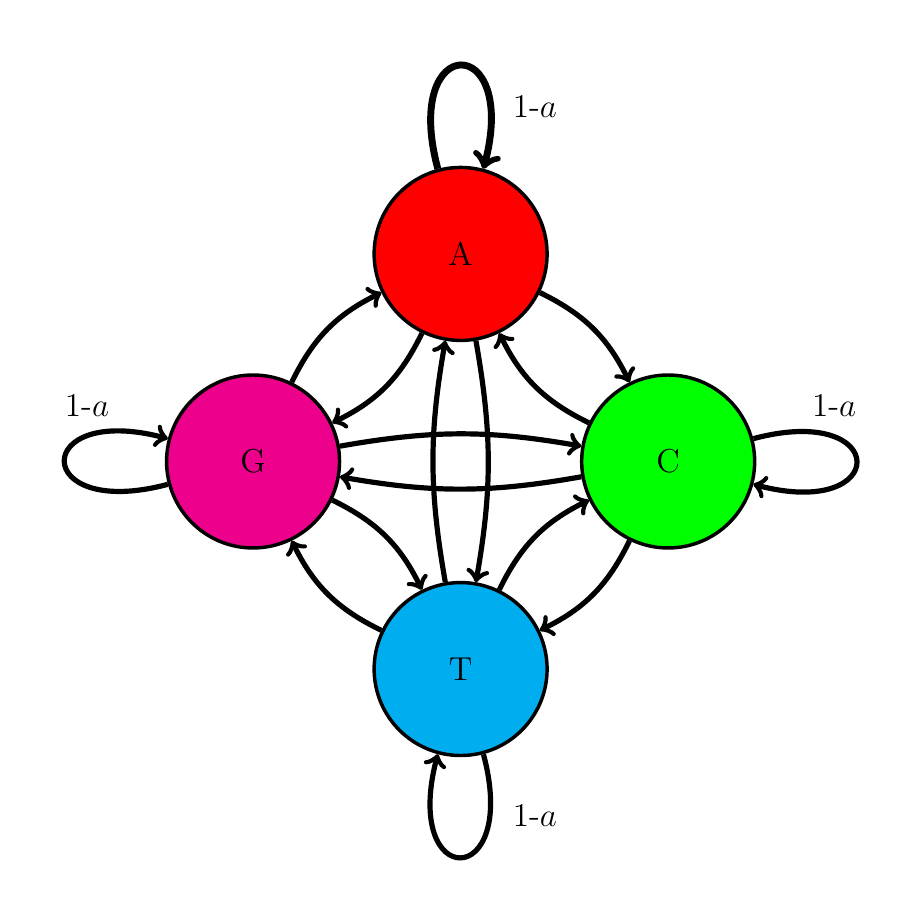
\begin{tikzpicture}
[every node/.style={inner sep=0pt}]
\node (1) [circle, minimum size=62.5pt, fill=red, line width=1.25pt, draw=black] at (187.5pt, -75.0pt) {\textcolor{black}{\large A}};
\node (4) [circle, minimum size=62.5pt, fill=cyan, line width=1.25pt, draw=black] at (187.5pt, -225.0pt) {\textcolor{black}{\large T}};
\node (3) [circle, minimum size=62.5pt, fill=magenta, line width=1.25pt, draw=black] at (112.5pt, -150.0pt) {\textcolor{black}{\large G}};
\node (2) [circle, minimum size=62.5pt, fill=green, line width=1.25pt, draw=black] at (262.5pt, -150.0pt) {\textcolor{black}{\large C}};
\draw [line width=1.875, ->, color=black] (1) to  [in=116, out=334] (2);
\draw [line width=1.875, ->, color=black] (2) to  [in=296, out=154] (1);
\draw [line width=1.875, ->, color=black] (1) to  [in=26, out=244] (3);
\draw [line width=1.875, ->, color=black] (3) to  [in=206, out=64] (1);
\draw [line width=1.875, ->, color=black] (3) to  [in=116, out=334] (4);
\draw [line width=1.875, ->, color=black] (4) to  [in=296, out=154] (3);
\draw [line width=1.875, ->, color=black] (4) to  [in=206, out=64] (2);
\draw [line width=1.875, ->, color=black] (2) to  [in=26, out=244] (4);
\draw [line width=1.875, ->, color=black] (1) to  [in=80, out=280] (4);
\draw [line width=1.875, ->, color=black] (4) to  [in=260, out=100] (1);
\draw [line width=1.875, ->, color=black] (3) to  [in=170, out=10] (2);
\draw [line width=1.875, ->, color=black] (2) to  [in=350, out=190] (3);
\draw [line width=2.5, ->, color=black, loop above] (1) to (1);
\draw [line width=1.875, ->, color=black, loop right] (2) to (2);
\draw [line width=1.875, ->, color=black, loop below] (4) to (4);
\draw [line width=1.875, ->, color=black, loop left] (3) to (3);
\node at (214.375pt, -21.875pt) {\textcolor{black}{\large 1-$a$}};
\node at (322.5pt, -130.0pt) {\textcolor{black}{\large 1-$a$}};
\node at (214.375pt, -278.125pt) {\textcolor{black}{\large 1-$a$}};
\node at (52.5pt, -130.0pt) {\textcolor{black}{\large 1-$a$}};
\end{tikzpicture}

\end{document}